% !TEX encoding = UTF-8
% !TEX program = pdflatex

\documentclass[a4paper]{report}
\usepackage[T1]{fontenc}
\usepackage[utf8]{inputenc}
\usepackage[english]{babel}
\usepackage{graphicx}
\usepackage{listings}
\usepackage{xcolor}
\definecolor{light-gray}{gray}{0.95}
\lstset{language=PHP,tabsize=2,backgroundcolor=\color{light-gray}}

\begin{document}

\begin{titlepage}
\centering
\vspace*{\stretch{1}}

\includegraphics{logoRomaTre.jpg}\\
\vspace*{\stretch{6}}
{\LARGE \bf Web Services Platform for the visualization of gene expression data\par}
\vspace{0.5cm}
{\Large Comparison between differential analysis\par} 
\vspace{2cm}
di\\
{\Large \em Chiara Bartalotta, Dario Santilli, Davide Bernardini\par}
\vspace*{\stretch{2}}
\date{\currenttime}
\today
\end{titlepage}

\tableofcontents

\chapter{Usage Case}
WEB-gene expression is a platform for the visualization of gene expression data. The platform offers different services basing on the type of user. Indeed, the users are distinguished between \emph{normal user} and \emph{super user}.
\begin{itemize}
   \item \textit{super user}: super user can benefit of advanced services. he is responsible for the management of the experiments: he can insert a new experiment or delete and modify one of the instance previously stored. Furthermore, the super user is able to enable a normal user to visualize an experiment. 
   \item \textit{normal user}: after the login phase, the normal user can display only the experiments for which viewing is enabled.
\end{itemize}

\section{Super user services}

\begin{figure}[htb] 
\begin{center}
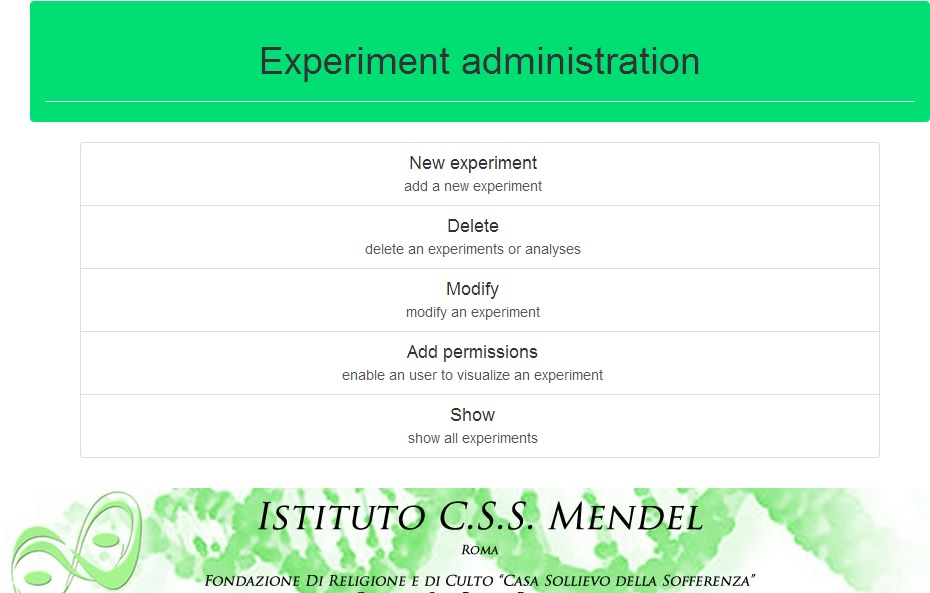
\includegraphics[scale=0.4]{figure/SUservices.jpg} 
\end{center}
\caption{Super user administration panel.}
\label{SUservices}
\end{figure}

As shown in Figure \ref{SUservices} , after the login, the platform allows the super user to access to different services. Indeed, the super user can choose among several options.

\subsection{Insert}
Through the \emph{insert} option, the user is able to store a new experiment with its relative analyses. In a first phase, the user defines the name of the new experiment, then he can choose the file with experiment's data and the system can upload it. 

\subsection{Delete and Modify}
The super user is able to delete an entire stored experiment with the \emph{delete} option, or he can only modify it. Indeed, with the \emph{modify} service, the super user can change the data of experiments. In a first phase, the user selects an existing  experiment that he want to modify, then he chooses the file with new data and the system updates the selected experiment.

\subsection{Add permission}
Another services that the platform provides to the super user  is the possibility to add permissions for the visualization of the experiments. A normal user, indeed, can see only the experiments for which he is enabled. A normal user can not visualize anything without the authorization of the super user.\\
Thought the \emph{add permission} option, the super user selects firstly the user for which to add permission and then the experiment to enable.

\section{Common service}
The main interest of the WEB-gene-expression users is to visualize the stored experiments. Therefore the primary service provided by the platform is the \emph{Show} option.\\
The 	\emph{Show} option is a common service between super user and normal user. However, a super user can visualize all the stored experiments, while a normal user can visualize only the ones for which he is enabled.

\subsection{Show}
When a user choose the \emph{show} option, he select the experiment that he want to visualize.\\
Each experiment is composed of several analyses thus the system offers the possibility to choose only the interesting ones. The two main features of each analyses are the \emph{p-value} and \emph{fold-change} values .\\
In order to shown only the analyses with user's desired characteristics, the platform provides three types of filters.

\begin{figure}[htb] 
\begin{center}
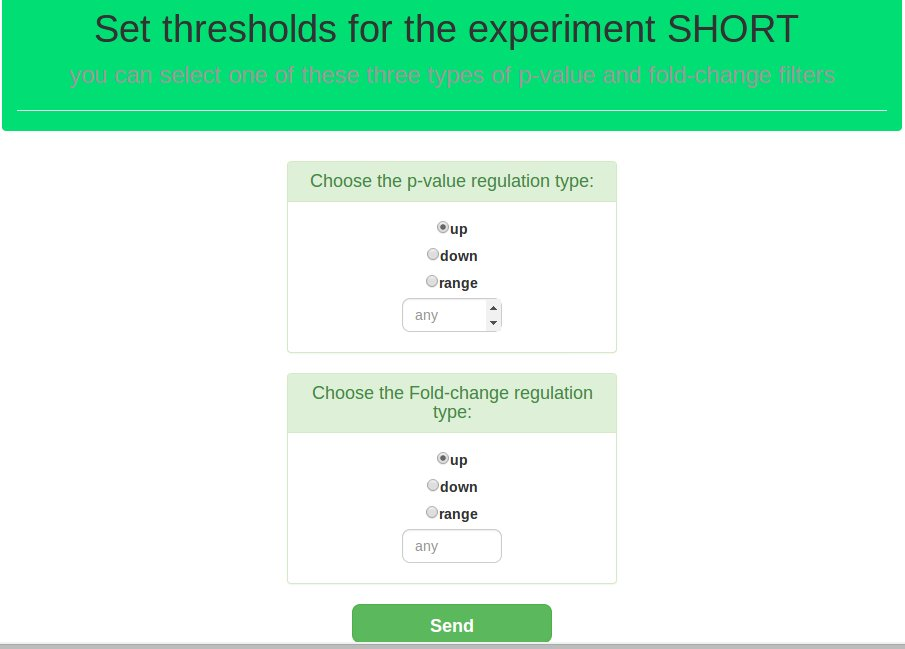
\includegraphics[scale=0.4]{figure/filters.jpg} 
\end{center}
\caption{Super user administration panel.}
\label{filters}
\end{figure}

As shown in figure \ref{filters}, the user can apply filters on the values of \emph{p-value} and \emph{fold-change}. If the user does not select a filter, the platform applies the default option and displays all the analyses without threshold on p-value and fold-change.

\begin{itemize}
    \item \textbf{p-value regulation type}: through this panel, the user can set a threshold on the p-value. Selecting \emph{up regulation}, the system will visualize the analyses with p-value greater than the specified threshold. Selecting \emph{down regulation}, the system will visualize the analyses with p-value less than the specified threshold. Finally, selecting \emph{range regulation} the system will visualize the analyses with p-value in the range of the threshold. For example, selecting \emph{range regulation} and threshold \emph{0.10} , the system shows analyses with p-value between -0.10 and +0.10.
    \item \textbf{fold-change regulation type}: analogously to the p-value regulation, the user can choose a filter on the \emph{fold-change} value. Also for the fold-change the user can define the threshold using \emph{up regulation} , \emph{down regulation} and \emph{range regulation}.
\end{itemize}

After that the user has selected a regulation option, the system shows the analyses that respect the user-defined threshold in a table.\\
As shown in figure \ref{table} , the first column of the table is the \emph{Gene} code and for each analysis there are two columns, one for the \emph{p-value} and another one for the \emph{fold-change}. The name of the analysis is specified over the p-value and fold-change field.\\

\begin{figure}[htb] 
\begin{center}
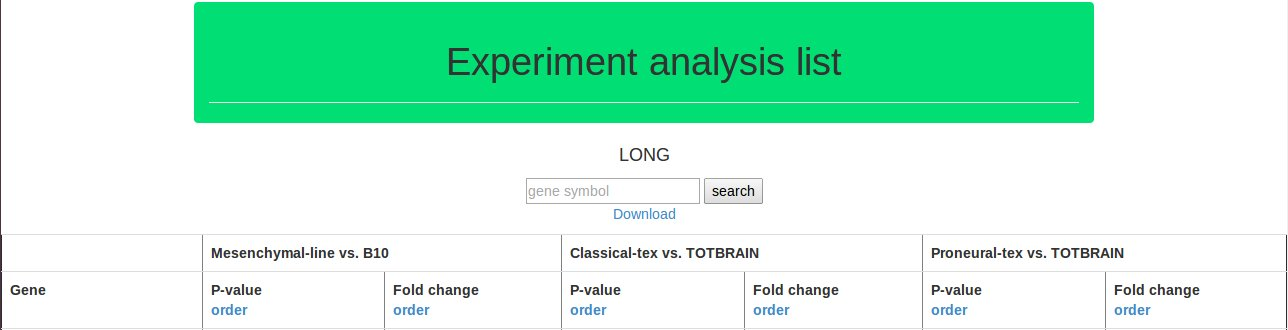
\includegraphics[scale=0.4]{figure/tableHeader.jpg} 
\end{center}
\caption{Super user administration panel.}
\label{tableHeader}
\end{figure}

The Figure \ref{tableHeader} shows that at any time the user can reorder the analyses based on the p-value or fold-change values by clicking on \emph{order}. By specifying the \emph{Gene code} in the \emph{search bar} , the user can visualize only the instance of the analyses relative to the specified gene.\\
The system provides the user also the possibility to download a file with the experiment data. As shown in Figure \ref{tableHeader}, the \emph{download} option is below the search field. By clicking on it, the user can save all the table in a \emph{.txt} file.


\begin{figure}[htb] 
\begin{center}
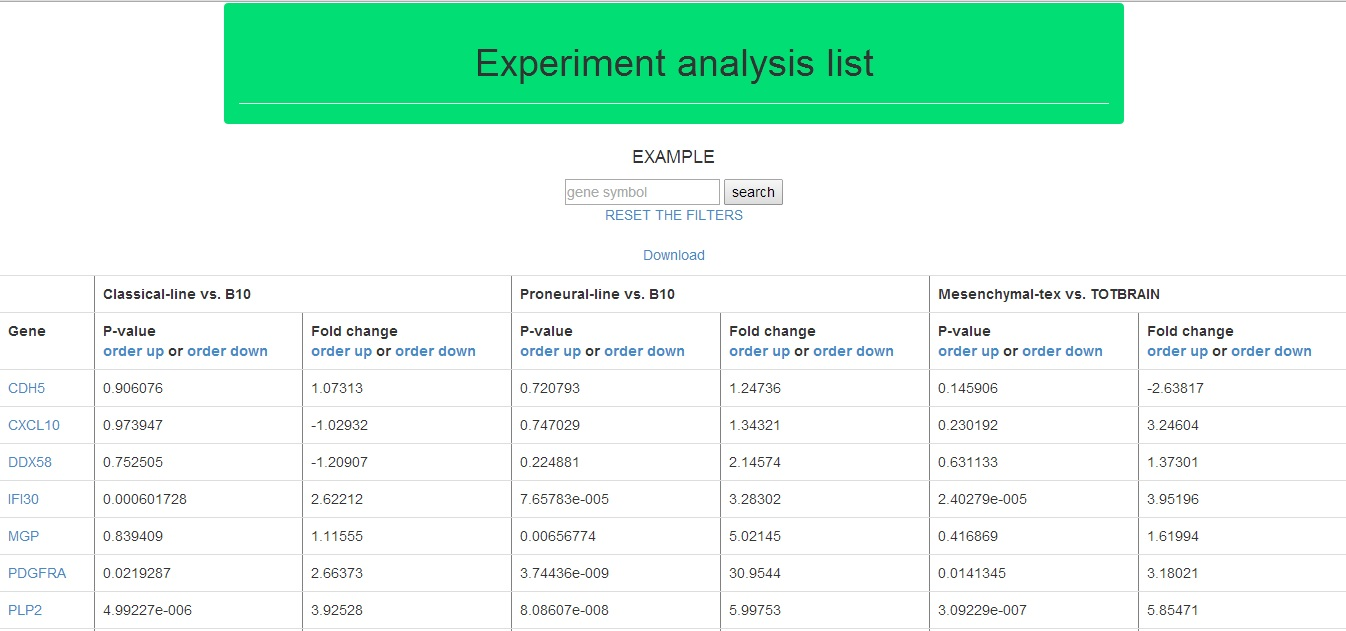
\includegraphics[scale=0.4]{figure/table.jpg} 
\end{center}
\caption{Super user administration panel.}
\label{table}
\end{figure}


\chapter{Technologies}
WEB-gene expression is developed as a web platform following the guide of the client-server architecture. The platform was built using JavaScript and jQuery to manage the client-side and the html page, and PHP and MySQL to manage the server-side. This chapter provides a description of these technologies and an explanation about how these technologies were used.

\section{Client-Server Architecture}

The Client-Server Architecture is a structure adopted to develop software applications. The aim of the Client-Server model is to divide the tasks of the application between server and client. The work of the Client is to request a service to a server which provides functions in order to respond to the request of the Client.\\
The browser is an example of Client. The browser connects itself to a Server that provides the information required by the user. In this way, the browser displays the response allowing the user to interact with this information. The program that responds to the browser request is an example of Server. It is listening to client requests, and it is always ready to provide the response.\\
The Figure \ref{clientServer} is a computer network diagram that shows the communication between clients and server by internet. In the figure, two clients are represented in order to indicate that the server receives the requests from multiple clients as described in section \ref{serverside}. 

\begin{figure}[htb] 
\begin{center}
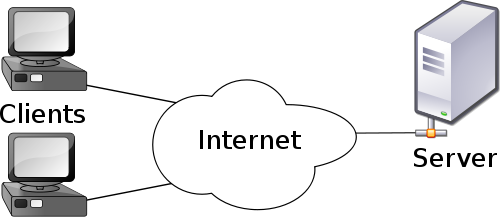
\includegraphics[scale=0.4]{figure/clientServer.png} 
\end{center}
\caption{Client-Server architecture.}
\label{clientServer}
\end{figure}

\subsection{Communication Protocol}

The Client side and the Server Side exchange message between each other using a Communication Protocol. A communication protocol defines rules about the syntax, the semantic and the synchronization of communication in order to manage the message exchange among computer systems.  Each message has a defined format, and its objective is to provoke a specific response from the receiver.\\

In WEB-gene-expression, the server side and the client side communicate through the HTTP protocol (HyperText Transfer Protocol) that is based on TCP/IP (Transmission Control Protocol / Internet Protocol). This protocol allows the server side and the client side to exchange ordered byte sequences.
\\In order to access the resource, the client side sends the server side a string of characters defined as URI (Uniform Resource Identifier). Each URI refers to a specific resource.

\subsection{Sever-Side}\label{serverside}

The server is always listening to the requests of the Clients. When a requests arrives, the Server provides the response by running an application able to satisfy the Client request.\\
The Server is able to satisfy many requests coming from different clients at the same time.\\
With regards to WEB-gene-expression, php is the language used to develop the server side. The framework adopted to create the web application in PHP is XAMPP.


\subsubsection{Server Tasks} 
In WEB-gene-expression, the server side has the task to manage the client requests by connecting the system to the database and providing the response data. \\
The database guarantees the data persistence while the server side organizes the application logic for managing of the operations with the data.\\

\subsubsection{The PHP language}\label{php}

The programming language used to develop the server side of WEB-gene-expression is PHP.\\

"PHP is a popular general-purpose scripting language that is especially suited to web development. Fast, flexible and pragmatic, PHP powers everything from your blog to the most popular websites in the world." \footnote{www.php.net}


Therefore, the main features of PHP meet WEB-gene-expression requirements for the implementation of the server side. The code is organized in classes following the principles of \emph{High Cohesion} and \emph{Low Coupling} described in "Applicare UML e i pattern" \cite{Craig Larman, Luca Cabibbo} . \\
The \emph{Low Coupling} pattern describes how to keep a low dependency among objects in order to guarantee a better usability of the code and a lower impact of the code changes.\\
The \emph{High Cohesion} pattern describes how to assign a specific, focused and comprehensible responsibility to each object in order to provide maintainability of the code.\\

\subsubsection{XAMPP}

XAMPP is an usefull environment for development of web applications in PHP. XAMPP aims at offering intuitive tools that allow the developer to create pure PHP web applications in a fast way \footnote{https://www.apachefriends.org/index.html}.\\
XAMPP is used to develop the server-side of WEB-gene-expression and his distribution contains not only PHP but also MySQL database.

\subsection{Database}

The database is responsible of information persistence. WEB-gene-expression has to operate a large amount of data coming from the experiment about differential analysis of gene expression data. In order to store these data, SICS use \emph{MySQL} as database.

\subsubsection{MySQL}

MySQL\footnote{http://www.mysql.it/} is a powerful, open source object-relational database system that runs on all major operating systems.
\\During the development phase, MySQL was chosen as WEB-gene-expression database for the following features. MySQL guarantees reliability, data integrity, correctness and stability. Furthermore, the extensible features and the large compatibility of MySQL are key features required by WEB-gene-expression. Due to these characteristics, WEB-gene-expression can be efficiently extend and reused in other systems.

\subsubsection{DataBase structure}

In an entity-relation database, the information is organized in different tables connected between each other through relations. Each table represents a concept of an entity and contains the instances of this entity. The \emph{entities} describe classes of objects with common properties but autonomous existence. The \emph{relations} represent the logic links between two or more entities.\\
The database in SICS is composed of five table which represent the entities of the application. \emph{Experiments} table collects the instances saved by the super user. It contains an univocal id, the name of the item, the date corresponding at the time when the experiment was loaded. The \emph{Analysis} table stores the differential analysis of an experiment. His columns are	univocal id, geneSymbol on which the analysis is done, p\_value , foldChange, the name of the analysis, the date an the id of the corresponding experiment. 
The \emph{Gene} table collects information about genes. This information are 	univocal id, geneSymbol, geneAssignment and refSeq.
\emph{Users} table collects the data regarding the users of the system. Each record contains the univocal id,name, surname, email, password and type of an user.
 Finally, the last table is the \emph{View Permission} table that collects the permissions of each user. With the two columns , id user and id experiment, this table stores the experiments that a normal user can visualize.\\

\paragraph{}The following logic schema describes the entity tables:
\begin{quote}
\item EXPERIMENT(\underline{id}, name, date) 
\item ANALYSIS(\underline{id}, geneSymbol, p\_value, foldChange, name, date, id\_experiment) with referential integrity between the \emph{id\_experiment} attribute and the \emph{EXPERIMENT} relation and between the \emph{geneSymbol} attribute and the \emph{GENE} relation.
\item GENE(\underline{id}, geneSymbol, geneAssignment, refSeq) 
\item USER(\underline{id}, name, surname, email, password, type) 
\item VIEWPERMISSION(\underline{id\_user}, \underline{id\_experiment})  with referential integrity between the \emph{id\_user} attribute and the \emph{USER} relation and between the \emph{id\_experiment} attribute and the \emph{EXPERIMENTS} relation.
\end{quote}

\subsubsection{JavaScript and jQuery}

\paragraph{JavaScript}
JavaScript is considered the most appropriate language for development of web applications.
 ``JavaScript is a lightweight, interpreted, object-oriented language with first-class functions, most known as the scripting language for Web pages, but used in many non-browser environments''. \footnote{https://developer.mozilla.org/en-US/docs/Web/JavaScript}\\
JavaScript syntax is modelled on Java and C syntax. JavaScript, indeed, is a language object-oriented and functional at the same time. Thus, it combines Java properties with C properties.\\
JavaScript allows the developer to program in a flexible way because it is a scripting interpreted and not-typed language. However, these features cause a disadvantage: the debugging phase is time-expensive. The compiled languages allow the debugging with an IDE, while, in JavaScript, the workload of the debugging weights on the developer that is responsible to find and understand the errors in the code.

\subparagraph{jQuery}
 WEB-gene-expression is a platform that provides the user an intuitive research experience. Therefore, it adopts technologies that allow a simple and familiar interaction between the user and the application.\\
jQuery\footnote{http://jquery.com/} is a JavaScript library that allows the implementation of several interactive functionalities. jQuery handles interaction events, such as mouse-clicks and text highlighting. It manages asynchronous HTTP requests to exchange data between the browser and the server. These requests allow the dynamic update of the web page, and the user does not need to reload the page. During the development of the client-side of WEB-gene-expression, the choice of jQuery allowed not only to manage asynchronous requests, but also to organize the user interface. \\

\chapter{Implementation}
This chapter discusses the implementation details of WEB-gene-expression platform. In order to generate an ordered code, the entire project is divided in different package. In this way, a better usability of the code is guaranteed. Furthermore, this development approach provides the maintainability of the project.

\section{MVC pattern} \label{mvc}

The development of WEB-gene-expression is based on the most important software architectural pattern: Model-view-controller. The MVC pattern is adopted for implementing web application in major programming languages.\\
This pattern is used to separate application's tasks.


  \paragraph{Model} The Model component implements the application core. It is responsible to manage data and the operations relative to them. Therefore, the Model defines the logical part of the application.
  \paragraph{View} The View component is responsible to show the data that model contains. It is responsible to manage the user interface. Through the View component, indeed, the user can interact with the system sending inputs. The system response is elaborated by the View that shows the output with a comfortable and comprehensible visualization for the user.
  \paragraph{Controller} The Controller allows the interaction between Model and View component and keeps them separate. It manage data flow into model object and update the view whenever data change \footnote{http://www.tutorialspoint.com/design\_pattern/mvc\_pattern.htm}.  

\
\\Following the Model-View-Controller pattern guidelines, the WEB-gene-expression code is divided as described above.

\section{Packages}

Each operation provided by the WEB-gene-expression platform is implemented in a classes and his concerns are divided in \emph{Controller, Logic and View} packages. 
The main implemented operation are to manage the user login, user sign in, choose operations, insert and delete experiments, enable view permission, show the analysis of an experiment, modify user profile.

\paragraph{Controller} This package stores the classes that implement the Controller component of the web application stored. Controller Packages implements the server side of the application, so the programming language used is PHP as described in \ref{php}.
\begin{lstlisting}[title={example of logoutController.php},frame=trBL]
include_once ('../template/cls_fast_template.php');
	
	session_start();
	$tlp = new FastTemplate("../view");
	if(isset($_SESSION['iduser'])) {
		$tlp->define( array('logout'=>"logout.html"));
		$tlp->assign("ACTION","logoutDoneController.php");
		$tlp->parse('STATE','logout');
	
		Header("Content-type: text/html");
		$tlp->FastPrint();
	}
	else {
		header("Location: pageUnauthorized.php");
	}
\end{lstlisting}



\paragraph{Logic} The classes representing the model component of the project are stored in the Logic Package. The Model component is a part of the application server-side and the language used is PHP.
\begin{lstlisting}[title={Fragment of logicUser.php},frame=trBL]	
class LogicUser extends Logic {
	var $user;
		function __construct() {
			parent::__construct();
			$this->user = null;	
		}
		public function __get($value) {
			return $this->$value;
		}
		public function __set($name,$value) {
			$this->$name = $value;
		}	
		...
\end{lstlisting}

\paragraph{View} This package stores the classes that implement the View component of the web application  are stored. The View component implement the client side of the application. View-classes are HTML pages with embedded JavaScript and jQuery.
\begin{lstlisting}[title={login.html's body.},frame=trBL]	
<div align="center">
	<nav class="navbar navbar-inverse"
	style="background-color:#01DF74; width:900px;
	margin-top:0px;" >
  		<div class="page-header">
  			<h1>Registation Successfully</h1>
		</div>
	</nav>
	{MESSAGE}<br><br>
</div>
<div id="footer" style="margin-top:300px;"align="center">
	<img src="http://localhost/workspace/WEB-gene-expression
	/gene-expression/bootstrap/img/footer.jpg">
</div>
\end{lstlisting}

\paragraph{Util} This package contains two PHP classes to manage the interactions between Logic component and database. These classes are indispensable to establish a connection and exchange data with the database.
\begin{lstlisting}[title={DTO.php class.},frame=trBL]	
class DTO {

	var $DTO;
	function __construct() {
		$this->DTO = array();
	}
	public function getValue($name) {
		if (isset($this->DTO[$name])) {
			return $this->DTO[$name];
		}
		else return "";
	}
	public function setValue($name, $value) {
		$this->DTO[$name] =$value;
	}
	public function remove($name) {
		$this->DTO[$name] = null;
	}
}
\end{lstlisting}

\paragraph{Template} The Template package store a cls\_fast\_template.php class. It is a PHP extension for managing templates and performing variable interpolation\footnote{http://fasttemplate.grafxsoftware.com/docs/default/\_cls\_fast\_template\_php.html}.
Using cls\_fast\_template.php class, the web-pages of WEB-gene-expression can be modeled dynamically by fitting their content on the user.

\paragraph{Bootstrap} This package contains the tools to manage the user interface and the data visualization. In order to make the user experience not only comprehensible but also captivating, WEB-gene-expression platform employs Twitter Bootstrap\footnote{http://getbootstrap.com/}. The Bootstrap folder contains two subfolder: JavaScript (js) and CSS. The first one contains the classes to manage the users interaction and the second one contains the style sheets. 

\chapter{Gene Expression}

Gene expression is the process by which information from a gene is used in the synthesis of a functional gene product. These products are often proteins, but in non-protein coding genes such as ribosomal RNA (rRNA), transfer RNA (tRNA) or small nuclear RNA (snRNA) genes, the product is a functional RNA. The process of gene expression is used by all known life - eukaryotes (including multicellular organisms), prokaryotes (bacteria and archaea), and utilized by viruses - to generate the macromolecular machinery for life. Several steps in the gene expression process may be modulated, including the transcription, RNA splicing, translation, and post-translational modification of a protein. Gene regulation gives the cell control over structure and function, and is the basis for cellular differentiation, morphogenesis and the versatility and adaptability of any organism. Gene regulation may also serve as a substrate for evolutionary change, since control of the timing, location, and amount of gene expression can have a profound effect on the functions (actions) of the gene in a cell or in a multicellular organism.
\\
\begin{figure}[htb] 
\begin{center}
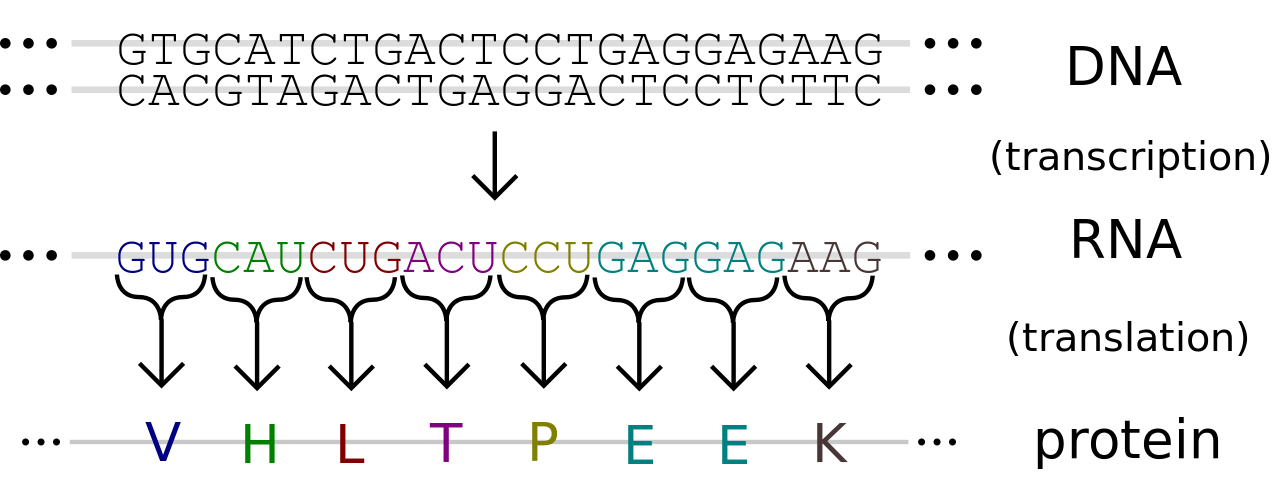
\includegraphics[scale=0.27]{figure/geneticCode.png} 
\end{center}
\caption{Transcription and translation.}
\label{geneExpression}
\end{figure}
\\
In genetics, gene expression is the most fundamental level at which the genotype gives rise to the phenotype. The genetic code stored in DNA is "interpreted" by gene expression, and the properties of the expression give rise to the organism's phenotype. Such phenotypes are often expressed by the synthesis of proteins that control the organism's shape, or that act as enzymes catalysing specific metabolic pathways characterising the organism.

\paragraph{Regulation}
Gene expression is tightly regulated by the cell. All steps of gene expression may be modulated, from the step of transcription of DNA to RNA, up to the post-translational modifications of the protein produced.\\
The regulation of gene expression is essential for the cell, because it allows its to control their internal and external functions.
\paragraph{Measure}
The expression of many genes is regulated at the base of the transcription, for example through the action of miRNA or siRNA, small RNA molecules can lead to the degradation of the transcript (high concentrations of mRNA are not always related to high concentrations of protein).\\
Anyhow, the amount of mRNA is a matter of considerable interest in the measurement of gene expression.
\section{DNA microarray}
There are various methodologies that allow for the screening of very large overall transcript of a cell. The method used by the CSS MENDEL institute is the one about DNA microarrays: through the use of supports that contain thousands of DNA probes complementary to the transcripts of the cell, this method is capable of providing simultaneous analysis of thousands of different mRNAs.\\

The DNA microarray technology is now a widely used tool 
in many biological and medical research. Its strength is to allow to measure the expression of thousands of genes simultaneously, in a single experiment.\\
The gene expression studies attempt to determine the quantity of a Messenger RNA (mRNA) transcribed in the biological system of reference: more quantities of RNA are produced, more protein are created. It is evident as the study of gene expression can be important to study those diseases, such as tumors, characterized by specific genetic alterations, from which depend the course of the disease and the efficacy of specific drugs. Only by comparing the gene expression of thousands of genes in individuals suffering from different diseases, it is possible to identify differentially expressed genes, and therefore potentially responsible the diversities in groups.\\
The statistical analysis of data obtained from microarray experiments is indispensable, not only for the identification of genes differentially expressed, but also for other biological targets not less important, such as the identification of co-regulated genes.\\
Genes are present in the DNA said "regulators", which lead to the formation of proteins that have the role of switches for the activation of a gene. Microarrays can also be used as a tool for classification between healthy subjects and patients, or between subclasses of a given disease. Often patients with the same disease may have different responses to different drug treatments. Through their molecular profile, and then through expression studies, it is seen that in reality, to the same disease could be divided into subclasses more pathological. This aspect makes it so extremely microarrays powerful both from a diagnostic and prognostic below that.\\

\begin{figure}[htb] 
\begin{center}
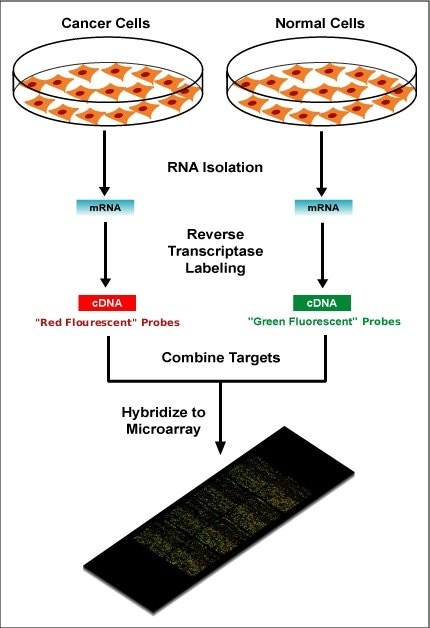
\includegraphics[scale=0.4]{figure/microarraySchema.jpg} 
\end{center}
\caption{Typical dual-colour microarray schema.}
\label{geneExpression}
\end{figure}

\end{document}
